\tikzstyle{rblock} = [rectangle, draw, text width=15em, text centered, inner sep=0pt, minimum height=2em, rounded corners]
\tikzstyle{line} = [draw, -latex']
\tikzstyle{arrow} = [thick,->,>=stealth]

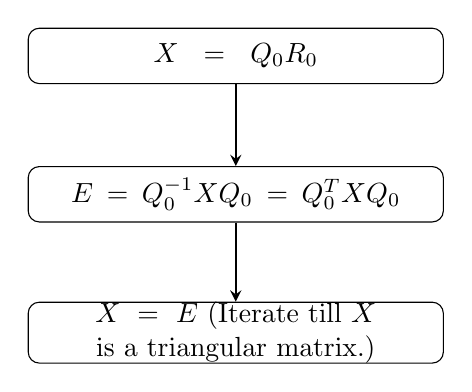
\begin{tikzpicture}[node distance = 5em, auto]
    \node (node7) [rblock] {$X = Q_0 R_0$};
    \node (node8) [rblock, below of = node7] {$E = Q_0^{-1} X Q_0 = Q_0^{T} X Q_0$};
    \node (node9) [rblock, below of = node8] {$X = E$ (Iterate till $X$ is a triangular matrix.)};
    \draw [arrow] (node7) -- (node8);
    \draw [arrow] (node8) -- (node9);
\end{tikzpicture}
